
\documentclass[12pt,onecolumn]{article}
\usepackage[brazilian]{babel}
\usepackage[utf8]{inputenc}
\usepackage{hyperref}
\usepackage[section]{placeins}
\usepackage{graphicx}
\usepackage{caption}
\usepackage{subcaption}
\usepackage{float}
\usepackage{framed,color}
\usepackage{wrapfig}

\begin{document}

% Title page.
\begin{titlepage}

    % Title info.
    \title{
        \bf
        \LARGE Apostila de \\
        \Huge  Infográficos
    }
    
    \author{Renan Teruo Carneiro \\ Wilson Kazuo Mizutani}
    
    % Print title.
    \maketitle
    
    % No numbering on this page.
    \thispagestyle{empty}
    
\end{titlepage}

\begin{center}
  Copyright (C) 2013 USPGameDev
\end{center}
\begin{figure}[ht]
  \centering
  
\includegraphics[width=\textwidth]{CC-BY.png}
\end{figure}

\vspace{300pt}

Escrito por:
\begin{itemize}
  \item \textbf{Renan Teruo Carneiro} \textit{(imano\_ob at uspgamedev.org)}
  \item \textbf{Wilson Kazuo Mizutani} \textit{(kazuo at uspgamedev.org)}
\end{itemize}

% Page break.
\clearpage

% Print table of contents.
\tableofcontents

% Page break.
\clearpage

\section{Introdução}
  Infográficos são representações gráficas e visuais de informação, dados ou
  conhecimento. Seu objetivo é apresentar informações complexas
  eficientemente\footnotemark.
  
  \footnotetext{
    \url{http://en.wikipedia.org/wiki/Infographic}, acesso em 21/04/2013.
  }
  
  Na realidade, Infográficos já existem há muitos anos. Mas foi só recentemente
  que a proliferação de ferramentas simples e livres trouxeram a criação de
  Infográficos para o alcance de um segmento maior da socedade. É no uso de
  algumas dessas ferramentas que essa apostila se concentra. Não é nosso
  objetivo dar nenhum curso sobre coleta e processamento de dados, mas sim sobre
  as possíveis maneiras de se apresentá-los em seu blog ou site de maneira
  simples e elegante.
  
  Mais particularmente, trabalharemos usando o software livre WordPress como
  ferramenta de blog para publicar os infográficos gerados pelas ferramentas que
  apresentaremos.

\clearpage
\section{\textit{Embedding}}
  Antes de mostrar as ferramentas de infográficos, vamos discutir como elas são
  integradas em um site. Usa-se uma técnica chamada \textit{Embedding}, que se
  traduz mais ou menos como "incorporar". E, de fato, o que essa técnica faz é
  incorporar mídias externas em um site qualquer.
  
  \subsection{Por que precisamos disso?}
    Os infográficos que faremos ficam hospedados no site que os gerou, porque
    eles que possuem a tecnologia para gerá-los. Além disso, serão infográficos
    relativamente interativos, portanto eles não são simples imagens para
    fazermos \textit{download}.
    
    Então, através do \textit{Embedding}, nós fazemos mídias complexas geradas
    em outros sites aparecerem naturalmente no nosso próprio site.
  
  \subsection{Como isso funciona?}
    Talvez você já saiba, mas todas páginas Web possuem um código fonte em
    \textit{HyperText Markup Language} (HTML). Tudo que aparece em uma página
    tem um código HTML por trás. Logo, se queremos colocar um infográfico em
    uma página, precisamos de algum tipo código HTML.
    
    É nesse ponto que entram as ferramentas de infografia Web. Elas não só os
    constroem, como os mantêm hospedados em seus sites e fornecem um trecho de
    código HTML para \textit{Embedding}, isso é, para colocarmos no nosso site.
    Basta copiar tal trecho e colá-lo no código do site, e pronto!
    
  \subsection{Onde eu acesso o código HTML do meu site? Como eu faço um site?}
    Normalmente, contrata-se um \textit{WebMaster} para criar uma página Web, e
    ele fornece um meio de inserirmos código HTML nele. Mas, para simplificar
    essa apostila, e manter o foco no que realmente interessa, usaremos a
    ferramenta de blog WordPress, que faz tudo isso para a gente.
    
    Nesse caso, você tem duas opções: criar um blog hospedado em
    \url{www.wordpress.com}, ou pedir para os monitores do curso criarem um
    para você\footnotemark. Uma vez que você tenha seu próprio WordPress, você
    poderá inserir código HTML nos seus \textit{posts} do blog, apresentando os
    infográficos que quiser.
    
    \footnotetext{
      Normalmente no endereço \url{www.uspgamedev.org/cursos/wordpress/}.
    }

\clearpage
\section{Ferramentas de uso geral}
  \subsection{Datawrapper}
     \textbf{Endereço: \url{http://datawrapper.de/}}
    
    %%Intro
    O Datawrapper é um serviço web voltado para a criação e manutenção de
    infográficos dos mais diversos tipos, relativamente interativos e com
    aparência profissional. Seu uso não exige nenhum tipo de conhecimento de
    design, apenas uma noção elementar de manipulação de planilhas. É possível
    se cadastrar no site e usar os serviços como disponibilizados, ou instalar
    sua própria instância do Datawrapper para maior personalização dos
    infográficos. Não cobriremos essas opções extras aqui, porém.
    %%Uso
    
    Tendo uma conta no site, para criar um infográfico, basta clicar no botão 
    "Create a Chart". O primeiro passo é entrar com os dados. Os dados podem ser 
    um arquivo .csv (Comma Separated Values) ou dados copiados e colados a partir
    de um editor de planilhas, como o Microsoft Excel ou o LibreOffice Calc.
    %%Exemplo de dados
    %%Tela com o resultado
    
    Logo em seguida, você poderá rever os dados para confirmar se eles foram
    reconhecidos corretamente. Você também pode informar ao serviço se a primeira
    linha e colunas são labels, se as séries de dados se encontram nas linhas ou
    nas colunas, e algumas outras opções de formatação nesse ponto. Também é
    possível creditar a fonte original dos dados, ou mesmo disponibilizá-los agora.
    %%Screenshot
    
    Feito isso, você deve estar na parte de visualização. Primeiro você deve escolher
    o tipo de gráfico a ser usado (Colunas, linhas, pie charts, etc). Se os dados não
    estiverem na disposição esperada, aqui é possível transpor os dados (ou seja, se
    você errou na hora de informar a disposição das séries de dados, dá pra arrumar 
    aqui). Aqui também é onde se nomeia o gráfico, e onde se coloca a descrição do
    mesmo. É possível também destacar uma série de dados em particular. Por fim, 
    é nessa parte em que você pode escolher as cores usadas, além de diversas outras
    opções visuais do gráfico.
    
    Finalmente, temos o gráfico pronto. Agora falta apenas publicar. Na última etapa,
    você tem o gráfico final, um link para o gráfico e o código html para emebedding
    do mesmo.
    
    Se quiser, você ainda pode modificar os gráficos já publicados. Eles se encontram
    em "My Charts". Lembre-se de republicá-los caso tenha modificado alguma coisa.
    %%Exemplo?

  \subsection{Infogram}
    \textbf{Endereço: \url{http://infogr.am/}}
    
    Infogram é um site de serviço Web voltado para a criação e manutenção de
    infográficos dos mais diversos tipos, relativamente interativos e com
    aparência profissional. Seu uso não exige nenhum tipo de conhecimento de
    design, apenas uma noção elementar de manipulação de planilhas. O site fornece
    um cadastro gratuito, com possibilidade de adquirir uma conta "Pro" para ter
    acesso a funcionalidades avançadas.
    
    Uma vez feita uma conta, é possível começar imediatamente a fazer
    infográficos. Na verdade, o site permite você criar um \textit{layout}
    bastante completo contendo um ou mais infográficos, textos, citações, imagens,
    mapas e vídeos. Também existem vários temas para esses \textit{layouts}.
    
    Na primeira vez que você entrar, o Infogr.am mostrará um esquema rápido
    explicando o que é cada ferramenta. Não são muitas, é bem simples de entender.
    A interface é dividida em quatro partes:
    
    \begin{itemize}
      \item
        \textbf{Menu lateral esquerdo:}
        Controle da conta, acesso à biblioteca pessoal de
        infográficos.
      \item
        \textbf{Menu lateral direito:}
        Adiciona elementos no \textit{layout} que você quer
        publicar, em particuar cria os infográficos.
      \item
        \textbf{Menu superior:}
        Configurações do \textit{layout}, prévia visual do resultado,
        \textit{download} (funcionalidade para contas Pro) e compartilhar. É nessa
        última opção ("\textit{share}") que você poderá obter o código HTML para
        incorporar sua produção no seu site.
      \item
        \textbf{Editor visual do \textit{layout}:}
        Aqui você pode posicionar os elementos do seu \textit{layout}, escrever
        textos neles e colocar uma nota de \textit{Copyright}. Quando você clicar
        duas vezes em um infográfico, um menu de edição aparecerá para você mudar
        as configurações e os dados usados por ele.
    \end{itemize}
    
    Quando você cria um novo infográfico no seu \textit{layout}, você pode
    escolher dentre os diversos tipos que o Infogr.am fornece, como gráficos de
    linha, gráficos de setor, gráficos de barra, gráficos de espalhamento e
    muito outros. Alguns possuem variações, e todos podem ter suas cores
    modificadas. Essa última opção e outras aparecem no menu de edição do
    infográfico, que, como dita acima, aparece quando você clica duas vezes
    nele.
    
    No menu de edição do infográfico, você pode colocar os dados que o Infogr.am
    precisa para gerá-lo e controlar outras opções do visual em geral da
    produção. Essas opções dependem do tipo de infográfico. Fora isso, você
    também pode criar mais conjuntos de dados - e o infográfico gerado terá uma
    opção interativa de alternar entre os conjuntos de dados apresentados -,
    carregar dados a partir de arquivos em seu computador, e alterar o tamanho e
    as cores do infográfico apresentado.
    
    \begin{figure}[ht]
      \centering
      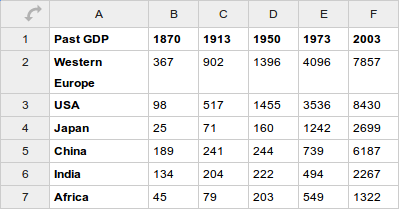
\includegraphics[width=.9\linewidth]{infogram-sample-spreadsheet.png}
      \caption{
        \footnotesize
        \it
        Exemplo de planilha que o Infogr.am usa para gerar gráficos de linha.
      }
      \label{fig:infogram-sample-spreadsheet}
    \end{figure}
    
    Os dados usados pelos infográficos devem ser fornecidos em uma planilha, o que
    é bastante conveniente. No entanto, esses dados precisam já estar processados
    e distribuídos da maneira que o Infogr.am espera. Por exemplo, um gráfico de
    linhas espera por uma tabela com: uma coluna com identificadores para cada
    linha do gráfico, e várias colunas com os valores associados acada
    identificador ao longo do tempo. Isso fica mais claro na Figura
    \ref{fig:infogram-sample-spreadsheet}. O gráfico resultante está na Figura
    \ref{fig:infogram-sample-chart}.
    
    Para passar uma planilha para o Infogr.am, basta copiar a parte desejada
    dela em um editor de planilhas de sua escolha e colá-la no menu de edição do
    infográfico. Ou você pode usar a opção de carregar de um arquivo em seu
    computador. Note que se a planilha carregada não estiver com a disposição
    que o Infogr.am espera, o resultado será inesperado.
    
    \begin{figure}[ht]
      \centering
      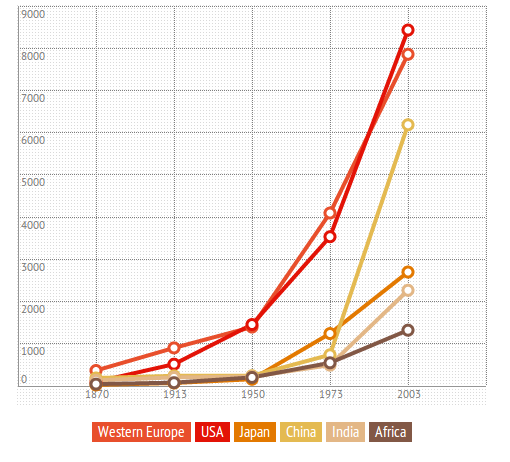
\includegraphics[width=.9\linewidth]{infogram-sample-chart.png}
      \caption{
        \footnotesize
        \it
        Gráfico de linha resultante da planilha da Figura
        \ref{fig:infogram-sample-spreadsheet}.
      }
      \label{fig:infogram-sample-chart}
    \end{figure}

\clearpage
\section{Ferramentas de uso específico}
  Às vezes queremos um tipo mais específico de Infográfico, e serviços Web de
  propósito geral nesse aspecto podem não ter tudo que a gente quer nesses
  casos. Essa seção dedica-se a explicar alguns outro sites de Infográfico de
  uso mais específico, como geradores especializados de "Word Clouds", por
  exemplo.

  \subsection{Google Trends}
    \textbf{Endereço: \url{http://www.google.com/trends/}}
    Google Trends é um site do Google que fornece estatísticas e infográficos
    sobre chaves de busca usadas pelas pessoas no site principal deles. Por
    exemplo, você pode pedir as Trends da busca "\textit{cats}", e o Google
    Trends mostrará uma página com diversas estatísticas sobre essa busca,
    como frequência ao longo do tempo, distribuição geográfica e termos
    relacionados.
    
    Cada um dos infográficos na página apresentada tem uma opção "Embed". Ela
    abre uma janela para você configurar o tamanho que você deseja que o
    infográfico tenha na sua página (em pixels) e fornece o código HTML
    correspondente. O uso do Google Trends é bem direto e específico mesmo.

  \subsection{Wordle}
    \textbf{Endereço: \url{http://www.wordle.net/}}
    

\end{document}
